\documentclass[border=10pt]{standalone}

\usepackage{tikz}
\usepackage{tikzsymbols}
\usetikzlibrary{calc,patterns,shapes.geometric}

\def\centerarc[#1](#2)(#3:#4:#5){\draw[#1] ($(#2)+({#5*cos(#3)},{#5*sin(#3)})$) arc (#3:#4:#5);}

\begin{document}
	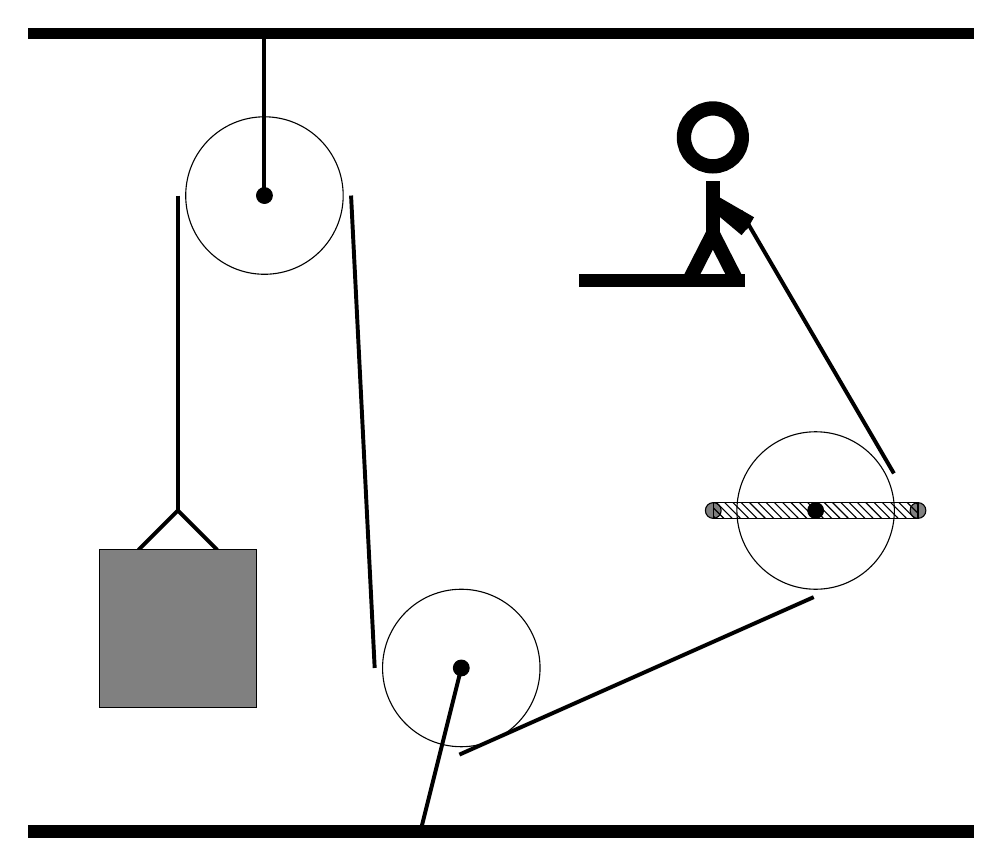
\begin{tikzpicture}
		%%%%% START %%%%%
		\draw[fill=black] (-2, 10) rectangle (10, 10.125);
		
		\draw (1, 8) circle (1);
		\draw[fill=black] (1, 8) circle (0.1);
		\draw[line width=0.5mm] (1, 10) -- (1, 8);
		
		\draw (3.5, 2.0) circle (1);
		\draw[fill=black] (3.5, 2.0) circle (0.1);
		\draw[line width=0.5mm] (3.5, 2.0) -- (3.0, 0);
		
		\draw[fill=white](8, 4.0) circle (1);
		\draw[fill=black] (8, 4.0) circle (0.1);
		\draw[fill=black!50] (9.3, 4.0) circle (0.1);
		\draw[fill=black!50] (6.7, 4.0) circle (0.1);
		\draw[pattern=north west lines, pattern color=black] (6.7, 4.1) rectangle (9.3, 3.9);
		
		\draw[line width=0.5mm](-0.6, 3.5) --  (-0.1, 4.0) -- (0.4, 3.5);
		\draw[fill=black!50] (-1.1, 3.5) rectangle (0.9, 1.5);
		
		\draw[line width=0.5mm](-0.1, 8) -- (-0.1, 4.0);
		\centerarc[line width=0.5mm](1, 8)(180:0:1.1)
		\draw[line width=0.5mm](2.1, 8) -- (2.4, 2.0);
		\centerarc[line width=0.5mm](3.5, 2.0)(180:300:1.1);
		\draw[line width=0.5mm](3.476, 0.9) -- (7.976, 2.9);
		\centerarc[line width=0.5mm](8, 4.0)(300:390:1.1);
		\draw[line width=0.5mm](8.994, 4.471) -- (7.05, 7.8);
		
		\node at (6.75, 8) {\Strichmaxerl[10][-220][-30]};
		\draw[fill=black] (5, 7) rectangle (7.1, 6.85);
		
		\draw[fill=black] (-2, 0) rectangle (10, -0.15);
		%%%%% END %%%%%
	\end{tikzpicture}
\end{document}